\chapter{Über diese \LaTeX{}-Vorlage}
Diese Vorlage ersetzt eine ältere Vorlage, die ich auf Basis von Professor Klaus Dohmens Vorlage erstellt hatte. Nachfolgend finden Sie eingige wichtige Informationen zu dieser aktuellen Vorlage vom Mai 2025. Eine gute und umfassende Einführung in \LaTeX{} finden sie im \href{https://de.wikibooks.org/wiki/LaTeX-Kompendium}{LaTeX-Kompendium}. Ein superkurze Einführung ist auch in meinem Buch \textit{Angewandte Bioinformatik} (Fig. \ref{fig:latex}) enthalten \citep{Wuenschiers2016kap12}.

\begin{figure}[h]
    \centering
    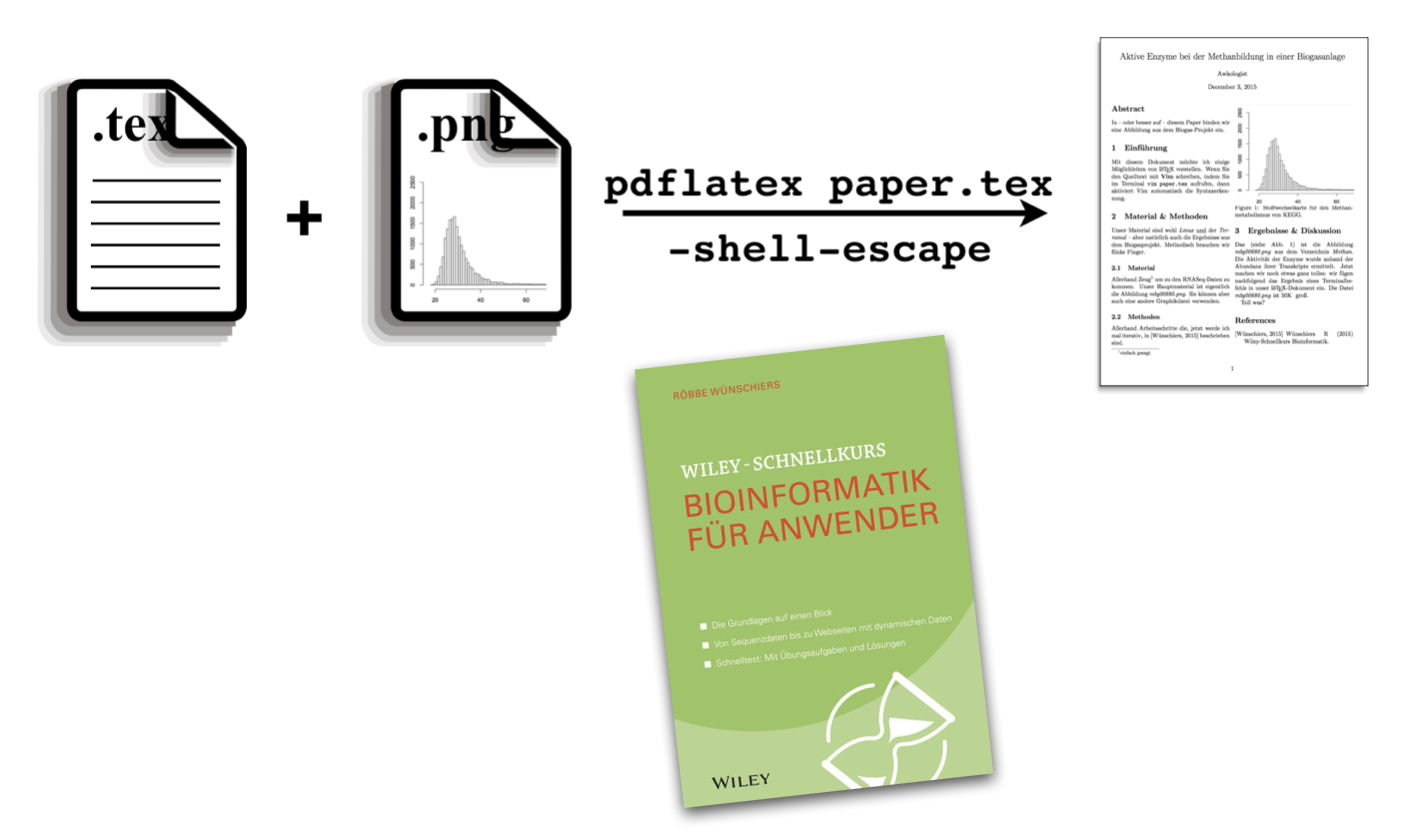
\includegraphics[width=.7\columnwidth]{fig-latex.png}
    \caption{Von \LaTeX{} zum PDF. Aus \citep{Wuenschiers2016}}.
    \label{fig:latex}
\end{figure}

Scheuen Sie sich nicht, mich auf Fehler hinzuweisen und Verbesserungsvorschläge einzubringen: \href{mailto:rw@biowasserstoff.de?subject=HSMW LaTeX-Vorlage}{Email}.

\alertinfo{Diese Beschreibung ist noch in Arbeit. Aktueller Stand: \today}


\section{Notwendige Dateien}
Diese Vorlage besteht aus mehreren Dateien, die alle im selben Verzeichnis liegen müssen. Sie können diese von meinem \href{https://github.com/awkologist/HSMW-Template-BioChem-Group}{GitHub-Repository} nach Click auf den Button \verb+<>Code+ $\rightarrow$ \textit{Download ZIP} als Dateiarchiv herunterladen und dann in \href{https://www.overleaf.com}{Overleaf} unter \textit{New Project} $\rightarrow$ \textit{Upload Project} importieren. Diese sind ...

\begin{tabular}{lp{.6\textwidth}}
\textit{hsmw-vorlage-rw.tex} & Die Hauptdatei, die die Formatierung bestimmt und Grunddaten enthält \\
\textit{mein-text.tex} & Datei, die ihren Haupttext enthält \\
\textit{fig-latex.png} & Eine Abbildung als Beispiel\\
\textit{magic-juggler.png} & Ein Logo als Beispiel\\
\textit{unterschrift.jpg} & Eine Unterschrift für die Selbstständigkeitserklärung als Beispiel\\
\textit{meine-abk.tex} & Datei mit den Begriffen und Definitionen für das Abkürzungsverzeichnis\\
\textit{meine-literatur.txt} & Datei mit ihrer Literatur im Bibtex-Format\\
\textit{hsmw-vorlage-rw.cls} & Die Style-Datei, welche die Formatierung bestimmt $\rightarrow$ \textbf{nicht editieren}\\
\textit{hsmw-biblatex.cfg} & Konfiguration für Literaturverzeichnis  $\rightarrow$ \textbf{nicht editieren}\\
\end{tabular}

\section{Protokoll, Beleg oder Abschlussarbeit}


\section{Formatierungsoptionen}
In der ersten Zeile der Vorlage \textit{hsmw-vorlage.tex} wird die Dokumentenklasse \textit{hsmw-class}  mit \verb+\documentclass[OPTIONEN]{hsmw-class}+ aufgerufen. Dabei stehen Ihnen zahlreichen OPTIONEN zur Verfügung:

%%%%%%%%%%%%%%%%%%%%%%%%%%%%%%%%%%%%%%   
    \chapter{Schnellstart: Die Vorlage nutzen}
	
	Um die Vorlage zu nutzen, müssen nur wenige grundlegende Entscheidungen getroffen werden, bevor es los gehen kann.
	Als erstes sollte die Art der Vorlage gewählt werden.
	Für Belegarbeiten setzen Sie die Klassenoption \enquote{\textit{thesis=paper}} (bzw. \enquote{\textit{thesis=shortpaper}}) und für Abschlussarbeiten verwenden Sie entweder für Diplomarbeiten \enquote{\textit{thesis=diploma}}, für Bachelorarbeiten\footnote{Bachelorarbeit ist der voreingestellte Standardwert, diesen müssen Sie demnach gar nicht explizit setzen.} \enquote{\textit{thesis=bachelor}} oder für Masterarbeiten \enquote{\textit{thesis=master}}.
	
	Anschließend müssen Sie relevante Felder in der Präambel setzen (dem Bereich vor dem eigentlichen Inhalt).
	Was Sie genau brauchen, können Sie in \cref{sec:macros} nachlesen -- es wird Ihnen aber auch im Dokument angezeigt, was noch fehlt.
	
	Damit sind die Vorbereitungen getroffen und es kann mit dem Inhalt los gehen.
	Auf dem Weg sollten Sie noch ein wenig Literaturarbeit nachweisen, wozu Sie im Allgemeinen noch Ihre Literatur einbinden müssen.
	Dazu ist die Verwendung des Pakets \enquote{\textit{biblatex}} dringend zu empfehlen -- mehr dazu in \cref{cha:bibliography}.
	
	Wenn Sie mit dem Erscheinungsbild der Vorlage noch nicht ganz zufrieden sind, können Sie über weitere Klassenoptionen und zusätzliche Befehle auch noch ein paar Anpassungen vornehmen.
	Dazu bieten Ihnen die \cref{cha:optionsAndCommands,cha:additionalChapters} weitere Hinweise.
	
	\section{Klassenoptionen}
	
	
	Wichtig ist für einen Beleg die entsprechende Klassenoption \enquote{\textit{thesis=paper}} zu setzen, damit das generelle Layout umgeschaltet wird.
	Weitere Klassenoptionen und Befehle können bei Bedarf in der Präambel ergänzt werden, um das Dokument den eigenen Bedürfnissen anzupassen.
	Zum Beispiel kann mittels der Klassenoption \enquote{\textit{faculty=cb}} die Fakultät CB und/oder mit dem Befehl \verb|\courseofstudy{Allgemeine und Digitale Forensik}| der Studiengang auf dem Titelblatt eingeblendet werden.
	
	
	Für eine Bachelorarbeit könnte die Klassenoption \enquote{\textit{thesis=bachelor}} sogar weggelassen werden, da dies als Standardeinstellung gesetzt ist.
	Beachten Sie bitte die Verwendung des zweisprachigen Titel-Befehls, der in der Vorlage für Abschlussarbeiten eine zusätzliche Titelseite nach internationalem Standard einfügt.
	Möchten Sie diese zusätzliche Titelseite unterdrücken, müssen Sie die Klassenoption \enquote{\textit{nosecondtitle}} setzen und dürfen dann die optionalen eckigen Klammern der zweisprachigen Befehle weglassen.
	
	\section{Fehler, Probleme oder Anpassungswünsche}
	
	Für allgemeine Probleme in der Umsetzung mit LaTeX, die so nichts mit der Vorlage zu tun haben, können Sie die offiziellen Kanäle verwenden:
	%
	\begin{itemize}
		\item \href{https://discord.com/channels/750860384126369822/765215969424834600}{HSMW Community Discord}
		\item \href{https://t.me/joinchat/Bxm0glfyeKXTM9OVlAhzJw}{Diskussionsgruppe in Telegram}
	\end{itemize}
	
	Falls Ihnen bei der Bearbeitung Fehler oder wünschenswerte Änderungen an der Vorlage selbst aufgefallen sind, nehmen Sie bitte Kontakt auf, um diese Probleme nicht nur für sich selbst zu lösen, sondern Alle daran teilhaben zu lassen und gemeinsam die Vorlage zu verbessern:
	%
	\begin{itemize}
		\item \href{https://git.hs-mittweida.de/hsmw-latex/hsmw-thesis/-/issues}{Problemverfolgung im GitLab}
		\item \href{mailto:schildba@hs-mittweida.de?subject=[LaTeX] Vorlage Abschlussarbeiten}{Direktkontakt per E-Mail}
	\end{itemize}
	
	
	
	\chapter{Verfügbare Optionen und Befehle}
	\label{cha:optionsAndCommands}
	
	Im Folgenden finden Sie eine Auflistung verfügbarer Klassenoptionen und Befehle, die direkte Auswirkungen auf die Dokumentenvorlage haben.
	
	\section{Klassenoptionen}
	
	Die Klassenoptionen dienen der initialen Konfiguration der Vorlage und sollten entsprechend zu Beginn des Dokuments gewählt werden, wenn eine Abweichung vom vordefinierten Standardverhalten gewünscht ist.
	Einige der Optionen sind voneinander abhängig oder beeinflussen sich gegenseitig, weswegen deren vorgeschlagene Reihenfolge nicht verändert werden sollte, um Fehler zu vermeiden.
	Einige Optionen nehmen Werte entgegen (mögliche Werte in Klammern), andere dienen nur als Schalter und besitzen keine zusätzlichen Parameter.
	Anwendungsbeispiele entnehmen Sie bitte den Beispieldokumenten.
	
	\begin{description}
		\item[language] (\textit{english}, \textit{ngerman}\footnote{\label{ftn:optionDefault}Wenn die Option nicht angegeben ist, ist dies der Standardwert (z.\,B. deutsch als Standardsprache).}\textsuperscript{,}\footnote{\label{ftn:optionDefaultValue}Wenn die Option ohne Wert angegeben ist, ist dies der Standardwert (z.\,B. \textit{language} anstatt \textit{language=ngerman}).}) Lädt die Standardsprache für das Dokument
		%
		\item[thesis] (\textit{paper}, \textit{shortpaper}, \textit{diploma}, \textit{bachelor}\footref{ftn:optionDefault}\textsuperscript{,}\footref{ftn:optionDefaultValue}, \textit{master}) Schaltet die Art der Vorlage um (Beleg oder Abschlussarbeit) und setzt Standardbezeichnungen und Layouteinstellungen
		\item[printmode] Verbirgt farbige Hyperlinks im Dokument (\textit{colorlinks=false}) und ändert die Farbdefinitionen zum Druckoptimierten CMYK-Farbmodell
		\item[draft] Aktiviert den Entwurfsmodus für schnelleres Kompilieren und Fehlerfinden
		\item[onesided] (\textit{true}\footref{ftn:optionDefaultValue}, \textit{false}\footref{ftn:optionDefault}) Wechselt zum einseitigen Dokumentenformat
		\item[nosecondtitle] Verbirgt die zweite Titelseite (englische Titelseite) für Abschlussarbeiten
		\item[compactlistof] (\textit{true}, \textit{false}\footref{ftn:optionDefault}\textsuperscript{,}\footref{ftn:optionDefaultValue}) Abbildungs- und Tabellenverzeichnis auf eine gemeinsam Seite
		\item[lotbeforelof] Tauscht die Reihenfolge von Abbildungs- und Tabellenverzeichnis
		\item[noauthorship] Verbirgt die Selbstständigkeitserklärung bzw. Eidesstattliche Erklärung
		%
		\item[colorlinks] (\textit{true}\footref{ftn:optionDefault}\textsuperscript{,}\footref{ftn:optionDefaultValue}, \textit{false}) Verwendet farbige Hyperlinks im Dokument
		\item[graduatedtoc] Nutzt ein eingerücktes Inhaltsverzeichnis (Standard: flach)
		\item[captionstyle] (\textit{default}\footref{ftn:optionDefault}\textsuperscript{,}\footref{ftn:optionDefaultValue}, \textit{minus}, \textit{flat}) Ändert den Stil der Nummerierungen von Über"=/Unterschriften (Standard mit Punkt getrennt, mit Minus getrennt oder kontinuierlich zählend)
		\item[smallromans] Verwendet kleingeschriebene römische Zahlen für die Seitennummerierungen der Verzeichnisse (Standard: große römische Zahlen)
		\item[glossaryhref] (\textit{true}\footref{ftn:optionDefault}\textsuperscript{,}\footref{ftn:optionDefaultValue}, \textit{false}) Schaltet Hyperlinks zum Glossar an oder aus
		\item[acronymhref] (\textit{true}\footref{ftn:optionDefault}\textsuperscript{,}\footref{ftn:optionDefaultValue}, \textit{false}) Schaltet Hyperlinks zum Abkürzungsverzeichnis an oder aus
		\item[acronymdots] (\textit{true}\footref{ftn:optionDefault}\textsuperscript{,}\footref{ftn:optionDefaultValue}, \textit{false}) Schaltet die Punktlinie im Abkürzungsverzeichnis an oder aus
		\item[symbolshref] (\textit{true}\footref{ftn:optionDefault}\textsuperscript{,}\footref{ftn:optionDefaultValue}, \textit{false}) Schaltet Hyperlinks zum Symbolverzeichnis an oder aus
		\item[symbolsdots] (\textit{true}\footref{ftn:optionDefault}\textsuperscript{,}\footref{ftn:optionDefaultValue}, \textit{false}) Schaltet die Punktlinie im Symbolverzeichnis an oder aus
		\item[fancy] Ändert mehrere Stiloptionen als inoffizielle Annäherung an das Corporate Design 2019
		%
		\item[theorembelow] Setzt einen Zeilenumbruch zwischen Theorem-Label und -Text (Standard: kleiner Abstand)
		\item[theoremdelim] (\textit{.}, \textit{:}, \textit{-}) Setzt den Trenner zwischen Theorem-Label und -Text (Standard: ohne)
		\item[sansmath] Verwendet eine serifenlose Schrift für mathematische Ausdrücke
		%
		\item[noautobuild] (\textit{true}\footref{ftn:optionDefaultValue}, \textit{false}\footref{ftn:optionDefault}) Deaktiviert die automatische Verarbeitung von Einträgen aus Abkürzungs"~, Glossar"~, Index"~, und Symbol-Verzeichnissen mittels \textit{makeindex} (manueller Programmaufruf notwendig)
		%
		\item[faculty] (\textit{inw}, \textit{cb}, \textit{wi}, \textit{sw}, \textit{me}) Lädt einen vordefinierten Fakultätsnamen (Standard: kein Name)
	\end{description}
	
	\textbf{Hinweise:}
	\begin{itemize}
		\item Verwenden Sie die voreingestellten Fakultätsnamen für Ihre Fakultät (\textit{faculty=cb}).
		\item Verwenden Sie für Belegarbeiten die Klassenoption \textit{thesis=paper} oder \textit{thesis=shortpaper} und setzen Sie ggf. die Art des Dokuments mittels \verb|\type{}| manuell neu.
		\item Nutzen Sie \textit{printmode}, bevor Sie das Dokument zum Druck geben, um das Hochschullogo in der richtigen Farbe zu erhalten und farbige Hyperlinks im Dokument zu unterdrücken.
	\end{itemize}
	
	
	
	\section{Standardbefehle für Autoren}
	\label{sec:macros}
	
	In \cref{tab:macros} ist eine Übersicht vordefinierter Befehle für die Konfiguration der Vorlage gegeben.
	Je nach verwendeten Klassenoptionen (Beleg oder Abschlussarbeit, Zweite Titelseite, etc.) und gewünschtem Dokumentenaufbau ist nur eine Auswahl davon nötig.
	Sollten einzelne Angaben fehlen, werden diese rot im Dokument hervorgehoben und zusätzlich als Warnung in die Log-Datei geschrieben.
	Einige der Befehle haben einen oder mehrere optionale Parameter, die im Folgenden kurz erläutert werden.
	Anwendungsbeispiele entnehmen Sie bitte den Beispieldokumenten.
	
	\begin{table}[!htb]
		\def\yes{notwendig}
		\def\no{-}
		\def\maybe{optional}
		
		\centering
		\caption{Verfügbare Befehle und deren Anwendungszwecke nach Dokumententyp.}
		\label{tab:macros}
		\begin{tabular}{llll}
			\toprule
			\textbf{Beschreibung} & \textbf{Beleg} & \textbf{Abschlussarbeit} & \textbf{Befehl(e)} \\
			\midrule
			\hyperref[cmd:type]{Art des Dokuments} & \yes & \yes & type \\
			\hyperref[cmd:author]{Autor(en)} & \yes & \yes & author, addauthor \\
			\hyperref[cmd:title]{Titel} & \yes & \yes & title \\
			\hyperref[cmd:subtitle]{Untertitel} & \maybe & \maybe & subtitle \\
			\hyperref[cmd:submissiondate]{Abgabedatum} & \yes & \yes & submissiondate \\
			\hyperref[cmd:defensedate]{Verteidigungsdatum} & \no & \yes & defensedate \\
			\hyperref[cmd:location]{Ort der Unterschrift} & \maybe & \maybe & location \\
			\hyperref[cmd:date]{Datum der Unterschrift} & \maybe & \maybe & date \\
			\hyperref[cmd:faculty]{Fakultät} & \maybe & \yes & faculty \\
			\hyperref[cmd:courseofstudy]{Studiengang} & \maybe & \yes & courseofstudy \\
			\hyperref[cmd:module]{Modul} & \maybe & \no & module \\
			\hyperref[cmd:seminargroup]{Seminargruppe} & \maybe & \yes & seminargroup \\
			\hyperref[cmd:email]{E-Mail} & \maybe & \no & email \\
			\hyperref[cmd:examiner]{Prüfer bzw. Betreuer} & \maybe & \yes & examiner, addexaminer \\
			\hyperref[cmd:abstract]{Referat} & \no & \yes & abstract \\
			\hyperref[cmd:preface]{Vorwort} & \no & \maybe & preface \\
			\hyperref[cmd:dedication]{Danksagung} & \no & \maybe & dedication \\
			\hyperref[cmd:nda]{Sperrvermerk} & \no & \maybe & nda \\
			\hyperref[cmd:frontispiece]{Frontispiz} & \no & \maybe & frontispiece \\
			\hyperref[cmd:partnerlogo]{Partnerlogo} & \maybe & \maybe & partnerlogo \\
			\bottomrule
		\end{tabular}
	\end{table}
	
	\textbf{Art des Dokuments:}\phantomsection\label{cmd:type}
	Setzt die Art des Dokuments auf den Titelseiten und in den bibliografischen Angaben.
	Wird durch die Klassenoption \textit{thesis} mit einem Standardwert vordefiniert (\textit{paper}=Belegarbeit, \textit{shortpaper}=Belegarbeit\footnote{Die Seitenumbrüche vor neuen Kapiteln werden bei \textit{shortpaper} entfernt und durch kleine Abstände ersetzt.}, \textit{diploma}=Diplomarbeit, \textit{bachelor}=Bachelorarbeit, \textit{master}=Masterarbeit).
	Der Befehl kann verwendet werden, um diesen Standardwert zu überschreiben.
	\begin{itemize}
		\item Für Belegarbeiten: \verb|\type{Deutsche Beschreibung}|
		\item Für Abschlussarbeiten: \verb|\type[Englisch]{Deutsch}|
	\end{itemize}
	
	\textbf{Autor:}\phantomsection\label{cmd:author}
	Setzt den Autor auf den Titelseiten, den bibliografischen Angaben und der Selbstständigkeitserklärung.
	Für den ersten Autor nutzen Sie bitte \verb|\author| und für zusätzliche Autoren \verb|\addauthor| (es kann auch für alle Autoren \verb|\addauthor| verwendet werden).
	Die vollständige Befehlssyntax beider Befehle ist:
	\newline
	{\small\verb|\author*(Anrede)[Titel]{Vorname}{Nachname}[Akad. Grad]<Unterschrift><Shift>|}
	\begin{itemize}
		\item Optional: *Sternversion schaltet zwischen der weiblichen und männlichen Anrede (Herr oder Frau) und passenden Labels (Autor wird zu Autorin) um
		\item Optional: (Anrede) überschreibt die vordefinierte Standardanrede (Herr bzw. Frau)
		\item Optional: [Titel] vor dem Vornamen (z.\,B. Dr. oder Prof. Dr. rer. nat.)
		\item Vorname
		\item Nachname
		\item Optional: [Akad. Grad] hinter dem Nachnamen (z.\,B. M.A. oder B.Sc.)
		\item Optional: <Unterschrift> gibt den Pfad zu einer Unterschriften-Datei an\footnote{Sollten Ihnen die Unterschriften in der Selbstständigkeitserklärung zu klein wirken, können Sie diese mit dem Befehl \texttt{\textbackslash{}setlength\{\textbackslash{}signatureHeight\}\{3\textbackslash{}baselineskip\}} in der Präambel vergrößern.}
		\item Optional: <Shift> schiebt die Unterschrift nach unten (z.\,B. \textit{0.5cm})
	\end{itemize}\vspace*{-\baselineskip}
	Beispiele für Autorenangaben:
	\begin{itemize}
		\item Ohne Titel und akademische Grade
		\begin{itemize}
			\item Männlicher Autor: \verb|\author{Holger Amadeus}{Herzog}|
			\item Weibliche Autorin: \verb|\author*{Frieda}{Fröhlich}|
			\item Mit Unterschrift: \verb|\author*{Frieda}{Fröhlich}<signatur-frieda.pdf>|
		\end{itemize}
		\item Mit Titel oder akademischen Grad
		\begin{itemize}
			\item Professor: \verb|\author[Prof.]{Egon}{Engelsbach}|
			\item Doktorin: \verb|\author*[Dr. rer. nat.]{Lucy}{Landgraf}<lucy.pdf>|
			\item Bachelorabschluss: \verb|\author{Sven}{Svenson}[B.Sc.]|
		\end{itemize}
		\item Mehrere Autoren:
		\begin{itemize}
			\item \verb|\author{Holger Amadeus}{Herzog}|
			\item \verb|\addauthor*{Frieda}{Fröhlich}<signatur-von-frieda.pdf>|
			\item \verb|\addauthor{Sven}{Svenson}[B.Sc.]|
		\end{itemize}
	\end{itemize}
	
	\textbf{Titel:}\phantomsection\label{cmd:title}
	Setzt den Titel auf den Titelseiten und in den bibliografischen Angaben.
	\begin{itemize}
		\item Für Belegarbeiten: \verb|\title{Deutsche Beschreibung}|
		\item Für Abschlussarbeiten: \verb|\title[Englisch]{Deutsch}|
	\end{itemize}
	
	\textbf{Untertitel:}\phantomsection\label{cmd:subtitle}
	Setzt den Untertitel auf den Titelseiten und in den bibliografischen Angaben.
	\begin{itemize}
		\item Für Belegarbeiten: \verb|\subtitle{Deutsche Beschreibung}|
		\item Für Abschlussarbeiten: \verb|\subtitle[Englisch]{Deutsch}|
	\end{itemize}
	
	\textbf{Abgabedatum:}\phantomsection\label{cmd:submissiondate}
	Setzt das Abgabedatum auf den Titelseiten und in den bibliografischen Angaben.
	Bitte nummerische Werte verwenden.
	Sollte nur das Jahr gesetzt sein, werden Monat und Tag als Annäherung aus dem aktuellen Datum verwendet.
	Soll anstatt der automatisierten Datumsroutinen einen fester Wert eingesetzt werden, kann die Sternvariante des Befehls genutzt werden.
	\newline
	\verb|\submissiondate*{Jahr}[Monat][Tag]|
	\begin{itemize}
		\item Optional: *Sternversion verwendet Jahr als Festwert (keine Datumsautomatik)
		\item Jahr der Verteidigung
		\item Optional: [Monat] der Verteidigung
		\item Optional: [Tag] der Verteidigung
	\end{itemize}
	
	\textbf{Verteidigungsdatum:}\phantomsection\label{cmd:defensedate}
	Setzt das Verteidigungsdatum (Jahr) auf den Titelseiten und in den bibliografischen Angaben.
	Bitte nummerische Werte verwenden -- für nicht-nummerische Werte kann die Sternversion des Befehls genutzt werden.
	Entfällt die Verwendung des Befehls, wird das Jahr des Abgabedatums genutzt.
	Diese Angabe ist nur für Abschlussarbeit relevant und findet keine Beachtung in Belegarbeiten.
	\newline
	\verb|\defensedate*{Jahr}[Monat][Tag]|
	\begin{itemize}
		\item Optional: *Sternversion verwendet Jahr als Festwert (keine Datumsautomatik)
		\item Jahr der Verteidigung
		\item Optional: [Monat] der Verteidigung (wird nicht mehr verwendet, Abwärtskompatibilität)
		\item Optional: [Tag] der Verteidigung (wird nicht mehr verwendet, Abwärtskompatibilität)
	\end{itemize}
	
	\textbf{Ort der Unterschrift:}\phantomsection\label{cmd:location}
	Setzt den Ort für die Selbstständigkeitserklärung bzw. die Eidesstattliche Erklärung.
	Als Standardwert ist hierfür Mittweida eingetragen.
	Der Befehl kann verwendet werden, um diesen Standardwert zu überschreiben.
	\newline
	\verb|\location{Ort}|
	
	\textbf{Datum der Unterschrift:}\phantomsection\label{cmd:date}
	Setzt das Datum für die Selbstständigkeitserklärung bzw. die Eidesstattliche Erklärung.
	Als Standardwert ist hierfür der aktuelle Zeitstempel (\verb|\today|) eingetragen.
	Der Befehl kann verwendet werden, um diesen Standardwert zu überschreiben.
	\newline
	\verb|\date{Datum}|
	
	\textbf{Fakultät:}\phantomsection\label{cmd:faculty}
	Setzt den Namen der Fakultät auf den Titelseiten und in den bibliografischen Angaben.
	Kann durch die Klassenoption \textit{faculty} mit einem Standardwert vordefiniert werden (\textit{inw}, \textit{cb}, \textit{wi}, \textit{sw}, \textit{me}).
	Der Befehl kann verwendet werden, um einen abweichenden Wert zu setzen, sollte die Klassenoption nicht verwendet werden.
	\begin{itemize}
		\item Für Belegarbeiten: \verb|\faculty{Deutsche Beschreibung}|
		\item Für Abschlussarbeiten: \verb|\faculty[Englisch]{Deutsch}|
	\end{itemize}
	
	\textbf{Studiengang:}\phantomsection\label{cmd:courseofstudy}
	Setzt den Studiengang auf den Titelseiten.
	\begin{itemize}
		\item Für Belegarbeiten: \verb|\courseofstudy{Deutsche Beschreibung}|
		\item Für Abschlussarbeiten: \verb|\courseofstudy[Englisch]{Deutsch}|
	\end{itemize}
	
	\textbf{Modul:}\phantomsection\label{cmd:module}
	Setzt den Namen des Moduls bzw. Kurses auf der Titelseite für Belege (\textit{paper}) und Kurzbelege (\textit{shortpaper}).
	\newline
	\verb|\module{Modulname}|
	
	\textbf{Seminargruppe:}\phantomsection\label{cmd:seminargroup}
	Setzt die Seminargruppe auf den Titelseiten.
	\newline
	\verb|\seminargroup{Seminargruppe}|
	
	\textbf{E-Mail:}\phantomsection\label{cmd:email}
	Setzt die E-Mail-Adresse auf der Titelseite.
	Mehrere E-Mail-Adressen können mittels \verb|\and| getrennt werden.
	Diese Angabe ist nur für Belegarbeiten relevant und findet keine Beachtung in Abschlussarbeiten.
	\newline
	\verb|\email{E-Mail-Adresse}|
	\newline
	\verb|\email{E-Mail-Adresse \and E-Mail-Adresse \and E-Mail-Adresse}|
	
	\textbf{Prüfer bzw. Betreuer:}\phantomsection\label{cmd:examiner}
	Setzt den Prüfer (Abschlussarbeiten) bzw. Betreuer (Belegarbeiten) auf den Titelseiten.
	Für den ersten Prüfer bzw. Betreuer nutzen Sie bitte \verb|\examiner| und für zusätzliche Autoren \verb|\addexaminer| (es kann auch für alle Prüfer bzw. Betreuer \verb|\examiner| verwendet werden).
	Für Abschlussarbeiten benötigen Sie genau zwei Prüfer --  einen Erstprüfer und einen Zweitprüfer.
	Die vollständige Befehlssyntax beider Befehle ist:
	\newline
	\verb|\examiner*[Titel]{Vollständiger Name}[Akad. Grad]|
	\begin{itemize}
		\item Optional: *Sternversion schaltet zwischen passenden Labels (Prüfer wird zu Prüferin) um
		\item Optional: [Titel] vor dem Namen (z.\,B. Dr. oder Prof. Dr. rer. nat.)
		\item Vollständiger Name
		\item Optional: [Akad. Grad] hinter dem Namen (z.\,B. M.A. oder B.Sc.)
	\end{itemize}\vspace*{-\baselineskip}
	Beispiele für Prüfer- bzw. Betreuerangaben:
	\begin{itemize}
		\item Professoren und Erstprüfer
		\begin{itemize}
			\item Professor: \verb|\examiner[Prof. Dr. rer. nat.]{Egon Engelsbach}|
			\item Doktorin: \verb|\examiner*[Dr. rer. nat.]{Lucy Landgraf}|
		\end{itemize}
		\item Zweitprüfer und Dozenten
		\begin{itemize}
			\item Dozentin mit Masterabschluss: \verb|\addexaminer*{Frieda Fröhlich}[M.A.]|
			\item Dozent mit Bachelorabschluss: \verb|\addexaminer{Sven Svenson}[B.Sc.]|
		\end{itemize}
	\end{itemize}
	
	\textbf{Referat:}\phantomsection\label{cmd:abstract}
	Setzt das Referat bzw. den \textit{Abstract} auf der Seite der bibliografischen Angaben.
	Sie können einen optionalen englischsprachigen \textit{Abstract} neben einem deutschsprachigen Referat angeben.
	Diese Angabe ist nur für Abschlussarbeit relevant und findet keine Beachtung in Belegarbeiten.
	\newline
	\verb|\abstract{Kurzreferat}|
	\newline
	\verb|\abstract[Englisch]{Deutsch}|
	\newline
	\verb|\abstract[Englisch]{Deutsch}[Trennzeichen]|
	
	\textbf{Vorwort:}\phantomsection\label{cmd:preface}
	Setzt ein Vorwort nach die Verzeichnisse und vor den Hauptteil der Arbeit.
	Sie können ein optionales Zitat inkl. Autor\footnote{\label{ftn:chapterquote}Das Zitat wird wie sonst auch üblich mittels \texttt{\textbackslash{}setchapterpreamble[u]\{\textbackslash{}dictum[\#2]\{\#1\}\}} gesetzt.} am Anfang des Abschnitts setzen.
	Diese Angabe ist nur selten für Abschlussarbeit relevant und sollte in Belegarbeiten komplett ignoriert werden.
	\newline
	\verb|\preface{Vorwort}|
	\newline
	\verb|\preface[Zitat][Zitatautor]{Vorwort}|
	
	\textbf{Danksagung:}\phantomsection\label{cmd:dedication}
	Setzt eine Danksagung nach die Verzeichnisse und vor den Hauptteil der Arbeit.
	Sie können ein optionales Zitat inkl. Autor\footref{ftn:chapterquote} am Anfang des Abschnitts setzen.
	Diese Angabe ist nur selten für Abschlussarbeit relevant und sollte in Belegarbeiten komplett ignoriert werden.
	\newline
	\verb|\dedication{Danksagung}|
	\newline
	\verb|\dedication[Zitat][Zitatautor]{Danksagung}|
	
	\textbf{Sperrvermerk:}\phantomsection\label{cmd:nda}
	Setzt einen Sperrvermerk auf der Seite der bibliografischen Angaben (nur relevant für Abschlussarbeit, keine Beachtung in Belegarbeiten).
	Übergeben Sie dem Befehl den Namen der Firma, deren Daten in der Arbeit präsentiert werden.
	\newline
	\verb|\nda{Firma mit sensiblen Daten}|
	
	\textbf{Frontispiz:}\phantomsection\label{cmd:frontispiece}
	Setzt die Rückseite des Schmutz- bzw. Schmucktitels.
	Kann für zusätzliche Informationen zum Verlag oder Druck verwendet werden.
	Diese Angabe ist nur selten für Abschlussarbeit relevant und findet keine Beachtung in Belegarbeiten.
	\newline
	\verb|\frontispiece{Frontispiz}|
	
	\textbf{Partnerlogo:}\phantomsection\label{cmd:partnerlogo}
	Setzt ein Partnerlogo neben das Hochschullogo auf die Titelseite.
	Das Logo wird mit einem vordefiniertem Abstand zum Hochschullogo eingefügt (Schutzraum) und auf dessen Größe skaliert.
	Ist das Partnerlogo in einem ungünstigen Format für diese Einschränkungen, kann es optional vergrößert werden.
	Anstelle einer Pfadangabe können auch alle Einstellungen manuell gesetzt werden.
	\newline
	\verb|\partnerlogo*[Höhe]{Pfad zur Logo-Datei}|
	\begin{itemize}
		\item Optional: *Sternversion interpretiert die Pfadangabe nicht als Pfad sondern als Inhalt
		\item Optional: [Höhe] überschriebt die vordefinierte Höhe
		\item Pfad zur Logo-Datei (oder Inhalt anstatt Logo-Datei)
	\end{itemize}
	
	\section{Erweiterte Befehle}
	
	In \cref{tab:hooks} können noch weitere Möglichkeiten eingesehen werden, wie individuelle Inhalte an vordefinierte Stellen im Dokument eingebracht werden können.
	
	\begin{table}[!htb]
		\centering
		\caption{Verfügbare \textit{Hooks} und deren Positionen im Dokument.}
		\label{tab:hooks}
		\begin{tabular}{lll}
			\toprule
			\textbf{Position im Dokument} & \textbf{Befehl} \\
			\midrule
			\hyperref[cmd:hookpreamble]{Letzte Konfigurationsmöglichkeit} & hookpreamble \\
			\hyperref[cmd:hooklof]{Text vor und nach dem Abbildungsverzeichnis} & hooklof \\
			\hyperref[cmd:hooklot]{Text vor und nach dem Tabellenverzeichnis} & hooklot \\
			\hyperref[cmd:hooklists]{Seite nach den Standardverzeichnissen} & hooklists \\
			\hyperref[cmd:hookbibliography]{Vordefiniertes Literaturverzeichnis} & hookbibliography \\
			\hyperref[cmd:hookpreauthorship]{Seite vor der Selbstständigkeitserklärung} & hookpreauthorship \\
			\hyperref[cmd:hooklastpage]{Seite nach der Selbstständigkeitserklärung} & hooklastpage \\	
			\bottomrule
		\end{tabular}
	\end{table}
	
	\textbf{Letzte Konfigurationsmöglichkeit:}\phantomsection\label{cmd:hookpreamble}
	Am Ende der Präambel, nach allen automatischen Konfigurationseinstellungen der Vorlage (z.\,B. zum Überschreiben vordefinierter Werte).
	\newline
	\verb|\hookpreamble{Konfigurationseinstellungen}|
	
	\textbf{Text vor und nach dem Abbildungsverzeichnis:}\phantomsection\label{cmd:hooklof}
	Allgemeine Bemerkungen zu allen Abbildungen oder dem Abbildungsverzeichnis an sich.
	\newline
	\verb|\hooklof{Text davor}{Text danach}|
	
	\textbf{Text vor und nach dem Tabellenverzeichnis:}\phantomsection\label{cmd:hooklot}
	Allgemeine Bemerkungen zu allen Tabellen oder dem Tabellenverzeichnis an sich.
	\newline
	\verb|\hooklot{Text davor}{Text danach}|
	
	\textbf{Seite nach den Standardverzeichnissen:}\phantomsection\label{cmd:hooklists}
	Für das Einfügen von weiteren benutzerdefinierten Verzeichnissen wie z.\,B. einem Symbol-, Formel-, oder Quelltextverzeichnis.
	Die Verzeichnisse werden nach dem Abbildungs- und Tabellenverzeichnissen und vor dem Abkürzungsverzeichnis eingefügt.
	Sollte die Klassenoption \enquote{\textit{compactlistof}} verwendet werden und zusätzliche Verzeichnisse eingebunden sein, wird die Überschrift der Verzeichnisse angepasst.
	\newline
	\verb|\hooklists[Kompakt][Normal]{Verzeichnisdefinitionen}|
	\begin{itemize}
		\item Optional: [Kompakt] Dieser Konfigurations-Teil wird ausgeführt, wenn die Klassenoption \enquote{\textit{compactlistof}} gesetzt ist
		\item Optional: [Normal] Dieser Konfigurations-Teil wird ausgeführt, wenn die Klassenoption \enquote{\textit{compactlistof}} nicht gesetzt ist
		\item Verzeichnisdefinitionen werden nach den optionalen Konfigurationen ausgeführt
	\end{itemize}
	
	\textbf{Vordefiniertes Literaturverzeichnis:}\phantomsection\label{cmd:hookbibliography}
	Das vordefinierte Literaturverzeichnis nimmt einige Einstellungen vor, damit die genutzte Literatur möglichst ohne Probleme dargestellt werden kann.
	Falls diese entfernt oder ersetzt werden sollen, kann der optionale Parameter des Befehls verwendet werden (z.\,B. falls nicht \textit{biblatex} verwendet wird).
	Weiterhin wird das Literaturverzeichnis standardmäßig in einem einzelnen großen Verzeichnis formatiert (\verb|\printbibliography|).
	Sollen z.\,B. mehrere Unterverzeichnisse für Bücher oder Online-Quellen erstellt werden, kann das Verhalten ebenfalls an dieser Stelle überschrieben werden.
	Das setzen von Werten in diesem Befehl überschreibt das Standardverhalten.
	\newline
	\verb|\hookbibliography[Einstellungen überschreiben]{Literaturausgabe}|
	
	\textbf{Seite vor der Selbstständigkeitserklärung:}\phantomsection\label{cmd:hookpreauthorship}
	Zusätzliche abschließende Verzeichnisse oder Bemerkungen.
	\newline
	\verb|\hookpreauthorship{Inhalt}|
	
	\textbf{Seite nach der Selbstständigkeitserklärung:}\phantomsection\label{cmd:hooklastpage}
	Inhalte nach allen vordefinierten Strukturen und Inhalten.
	Hier können ggf. fachspezifische Thesen untergebracht werden.
	\newline
	\verb|\hooklastpage{Inhalt}|
	
	Als Anwendungsbeispiel zum Hinzufügen eines zusätzlichen Quelltextverzeichnisses mit Hilfe der erweiterten Befehle kann \cref{lst:addLoL} herangezogen werden.
	
	\begin{lstlisting}[style=MyLatexStyle,caption={Beispielcode zum Hinzufügen eines Quelltextverzeichnisses mit dem Paket \textit{listings}.},label=lst:addLoL]
%%%%%%%%%% In der Präambel %%%%%%%%%%

\usepackage{listings} % Paket listings laden
\hooklists% Verzeichnis-Hook verwenden
	% Im Kompaktmodus: Überschrift als \section, nicht ins Inhaltsverzeichnis
	[\setuptoc{lol}{leveldown,notoc}]% lol = list of listings
	% Im Normalmodus: Überschrift als \chapter, ins Inhaltsverzeichnis aufnehmen
	[\setuptoc{lol}{totoc}]% lol = list of listings
	% Liste der Listings (lol) einfügen
	{\lstlistoflistings}

%%%%%%%%%% Später im Textteil %%%%%%%%%%

% Quellcode aus Datei einfügen
\lstinputlisting[float=htb,caption={Beschreibung},label=lst:example]{example.dat}
	\end{lstlisting}
	
	
	
	\chapter{Grundlegende Struktur und zusätzliche Abschnitte}
	\label{cha:additionalChapters}
	
	In \cref{tab:documentStructure} ist die grundlegende Struktur abgebildet, welche von der Vorlage bereitgestellt wird.
	Dabei sind einige Elemente in ihrer Existenz und Reihenfolge fest vorgegeben, andere hingegen können nach eigenem Bedarf und Geschmack verwendet werden.
	
	\begin{table}[!htb]
		\centering
		\caption{Grundlegende Struktur der Vorlage und verwendbare Elemente bei der Erstellung von Dokumenten mit der Vorlage.}
		\label{tab:documentStructure}
		\begin{tabular}{lllll}
			\toprule
			& \textbf{Beleg} & \textbf{Diplom} & \textbf{Bachelor} & \textbf{Master} \\
			\midrule
			Deckblatt & ja & ja & ja & ja \\
			Deutsches Titelblatt & nein & ja & ja & ja \\
			\hyperref[itm:englishTitle]{Englisches Titelblatt} & nein & ja & ja & ja \\
			\hyperref[itm:bibliographicData]{Bibliografische Angaben} & nein & ja & ja & ja \\
			\hyperref[itm:abstract]{Referat} & nein & ja & ja & ja \\
			\cmidrule(r){1-1}
			\cmidrule(l){2-5}
			Inhaltsverzeichnis & ja & ja & ja & ja \\
			Abbildungsverzeichnis & optional & optional & optional & optional \\
			Tabellenverzeichnis & optional & optional & optional & optional \\
			\hyperref[itm:acronyms]{Abkürzungsverzeichnis} & optional & optional & optional & optional \\
			\hyperref[itm:symbols]{Symbolverzeichnis} & optional & optional & optional & optional \\
			\cmidrule(r){1-1}
			\cmidrule(l){2-5}
			\hyperref[itm:preface]{Vorwort} & nein & optional & optional & optional \\
			\hyperref[itm:dedication]{Danksagung} & nein & optional & optional & optional \\
			\cmidrule(r){1-1}
			\cmidrule(l){2-5}
			\textbf{Inhalt} & ja & ja & ja & ja \\
			\hyperref[itm:appendix]{Anhang} & optional & optional & optional & optional \\
			\cmidrule(r){1-1}
			\cmidrule(l){2-5}
			\hyperref[itm:glossary]{Glossar} & optional & optional & optional & optional \\
			\hyperref[itm:bibliography]{Literaturverzeichnis} & ja & ja & ja & ja \\
			\hyperref[itm:index]{Stichwortverzeichnis} & optional & optional & optional & optional \\
			\hyperref[itm:soa]{Selbstständigkeitserklärung} & ja & Eid & Eid & Eid \\
			\bottomrule
		\end{tabular}
	\end{table}
	
	Im Folgenden werden einzelne Abschnitte näher beschrieben und deren Verwendungszweck kurz umrissen.
	
	\textbf{Englisches Titelblatt:}\phantomsection\label{itm:englishTitle}
	Die Verwendung eines zusätzlichen englischen Titelblatts stellt keine zwingende Notwendigkeit dar.
	In Hinblick auf den Gedanken der Internationalisierung und der freien Wissenschaft ist es aber durchaus eine Bereicherung für Abschlussarbeiten und sollte daher freiwillig zur Verfügung gestellt werden.
	
	\textbf{Bibliografische Angaben:}\phantomsection\label{itm:bibliographicData}
	Die bibliografischen Angaben gehören als fester Bestandteil zu jeder wissenschaftlichen Abhandlung.
	Die DIN 1505 Teil 1 schreibt deren einzelne Bestandteile, Reihenfolge und Trennzeichen vor.
	Die Angaben werden zur Indizierung der wissenschaftlichen Arbeit in einer Bibliografie verwendet.
	Die bibliografischen Angaben werden für Abschlussarbeiten automatisch erzeugt.
	
	\textbf{Referat:}\phantomsection\label{itm:abstract}
	Das (Kurz-)Referat (engl. \textit{Abstract}) kann als Klappentext der Arbeit verstanden werden.
	Es sollte den wesentlichen Inhalt der wissenschaftlichen Arbeit in wenigen Sätzen wiedergeben, ohne dabei nur den Titel der Arbeit zu wiederholen.
	Versuchen Sie mit Hilfe von informativen Aussagen den Inhalt der Arbeit zu erläutern.
	Das Referat kann in der Präambel mit \verb|\abstract{Referat}| gesetzt werden.
	Sie können auch im Sinne der Internationalisierung ein zusätzliches englischsprachiges Referat verfassen.
	
	\textbf{Abkürzungsverzeichnis:}\phantomsection\label{itm:acronyms}
	Das Abkürzungsverzeichnis ist eine alphabetische Liste von verwendeten fachlichen Abkürzungen und ihren Bedeutungen.
	Allgemein gebräuchliche Abkürzungen wie \enquote{etc.}, \enquote{usw.} oder \enquote{z.\,B.} werden nicht mit ins Abkürzungsverzeichnis aufgenommen.
	Grundsätzlich sollte eine zu kürzender Begriff bei der ersten Verwendung im Dokument ausgeschrieben werden und die Abkürzung in Klammern dahinter eingefügt werden.
	Anschließend kann im restlichen Dokument die Abkürzung verwendet werden.
	Zu verwendende Abkürzungen können in der Präambel definiert und im Text referenziert werden.
	%
	\begin{itemize}
		\item Definition in der Präambel: \verb|\newacronym{Label}{Abkürzung}{Bedeutung}|
		\item Verwendung im Text: \verb|\ac{Label}|
	\end{itemize}
	
	\textbf{Symbolverzeichnis:}\phantomsection\label{itm:symbols}
	Das Symbolverzeichnis ist eine Liste von verwendeten Symbolen und/oder Formelzeichen und deren Bedeutungen.
	Allgemein gebräuchliche Symbole wie \enquote{kg}, \enquote{m} oder \enquote{cm\textsuperscript{3}} werden nicht mit ins Symbolverzeichnis aufgenommen.
	Zu verwendende Symbole können in der Präambel definiert und im Text referenziert werden.
	%
	\begin{itemize}
		\item Definition in der Präambel: \verb|\newsymb{Label}{Symbol}{Name}{Bedeutung}|
		\item Verwendung im Text: \verb|\glssymbol{Label}|
	\end{itemize}
	
	\textbf{Vorwort:}\phantomsection\label{itm:preface}
	In herkömmlichen Abschlussarbeiten ist kein Vorwort notwendig.
	Das Vorwort umfasst normalerweise Bedingungen und Beweggründe für die Erstellung der wissenschaftlichen Arbeit und geht nicht auf den eigentlichen Inhalt ein.
	Es beinhaltet Hintergründe zu Ihrer Person und gibt der Arbeit eine persönliche Note.
	Ein Vorwort ist eher in zu veröffentlichen Büchern, Dissertationen und anderen Publikationen zu finden, die einem größeren Personenkreis zugänglich gemacht werden.
	Ein Vorwort kann mittels \verb|\preface{Vorwort}| in der Präambel erzeugt werden.
	
	\textbf{Danksagung:}\phantomsection\label{itm:dedication}
	Die Danksagung sollte sich konkret auf die wissenschaftliche Arbeit beziehen und kann z.\,B. verwendet werden, um Wertschätzung für eine finanzielle Unterstützung während der Bearbeitung, die Bereitstellung wertvoller Datensätze oder die Teilnahme an einer maßgeblichen Umfrage zu vermitteln.
	Achten Sie darauf, ob die erhaltene Unterstützung selbstverständlich ist oder über ein gewisses Maß hinaus geht und tatsächlich einer offiziellen Danksagung würdig ist.
	Beachten Sie weiterhin, dass Danksagungen in wissenschaftlichen Arbeiten häufig als unangemessen betrachtet und sogar zu Ihrem Nachteil interpretiert werden könnten.
	Eine Danksagung kann mittels \verb|\dedication{Danksagung}| in der Präambel erzeugt werden.
	
	\textbf{Anhang:}\phantomsection\label{itm:appendix}
	Ein Anhang kann verwendet werden, um Informationen in die Arbeit zu integrieren, welche das Verständnis der wissenschaftlichen Arbeit fördern, aber im Fließtext den Lesefluss zu stark stören würden.
	Dabei handelt es sich um Zusatzinformationen, die eine sinnvolle Ergänzung der Arbeit darstellen und daher an entsprechenden Stellen im Text referenziert werden sollten.
	Dazu gehören z.\,B. empirische Auswertungen, Interviews, Protokolle oder Herleitungen von Formeln.
	Der Anhang wird im Dokument vom Hauptteil mit der Anweisung \verb|\appendix| getrennt.
	
	\textbf{Glossar:}\phantomsection\label{itm:glossary}
	Das Glossar ist eine alphabetische Liste von verwendeten fachlichen Begriffen und ihren Bedeutungen.
	Dazu zählen mitunter Fachbegriffe, Fremdwörter und Eigennamen, die für einen durchschnittlichen Leser nicht zum Sprachgebrauch gehören.
	Ein Glossar ist in einer wissenschaftlichen Arbeit nicht erforderlich und entsprechende Definitionen können auch elegant in den Fließtext integriert werden.
	Glossar-Einträge können in der Präambel definiert und im Text referenziert werden.
	%
	\begin{itemize}
		\item Definition in der Präambel:\newline\verb|\newglossaryentry{Label}{name=Begriff,description={Beschreibung}}|
		\item Verwendung im Text\footnote{\label{ftn:glossaryCommands}Es kann mit \textbackslash{}Gls\{Label\} bzw. \textbackslash{}gls\{Label\} die Groß- und Kleinschreibung, sowie mit \textbackslash{}Glspl\{Label\} bzw. \textbackslash{}glspl\{Label\} die Mehrzahl des Begriffs verwendet werden.}: \verb|\Gls{Label}|
	\end{itemize}
	
	\textbf{Literaturverzeichnis:}\phantomsection\label{itm:bibliography}
	Das Literaturverzeichnis ist für eine wissenschaftliche Arbeit zwingend erforderlich, um eine Nachvollziehbarkeit der Argumentationsketten aus den verwendeten Quellen zu garantieren.
	Alles was nicht zum Allgemeinwissen gehört oder vom Autor stammt, muss durch eine Quelle belegt sein und jede im Text verwendete Quelle muss im Literaturverzeichnis vorkommen.
	Dabei schwanken die konkreten Anforderungen an die Literaturarbeit zwischen einzelnen Fachgebieten sehr stark (Zitierstil, Formatierung, Sortierung, etc.) -- informieren Sie sich dazu am besten bei Ihrem Betreuer.
	Weiterführende Informationen zum Thema Literaturarbeit finden Sie in \cref{cha:bibliography}.
	
	\textbf{Stichwortverzeichnis:}\phantomsection\label{itm:index}
	Ein Stichwortverzeichnis ist eine alphabetische Liste von verwendeten Schlagworten, welche mit Seitennummern belegt sind.
	Es dient dem Leser als Unterstützung bei der Suche nach bestimmten Wörtern.
	Ein Stichwortverzeichnis ist nicht erforderlich, kann allerdings durch die Verwendung des Befehls \verb|\index{Schlagwort}| an geeigneter Stelle im Text erzeugt werden.
	Hinweis: Der Befehl selbst ist nur eine Referenzstelle für das Stichwortverzeichnis und erzeugt keine Ausgabe im Text.
	
	\textbf{Selbstständigkeitserklärung und eidesstattliche Erklärung:}\phantomsection\label{itm:soa}
	Die Selbstständigkeitserklärung stellt eine schriftliche Bestätigung dar, dass der Autor die wissenschaftliche Arbeit selbstständig verfasst und verwendete Hilfsmittel und Literaturquellen ordnungsgemäß gekennzeichnet hat.
	Dadurch wird versichert, dass es sich bei der Arbeit nicht um ein Plagiat handelt.
	Für Abschlussarbeiten wird die Selbstständigkeitserklärung durch eine eidesstattliche Erklärung ersetzt.
	Dieser Eid ist rechtlich bindend und wird bei der Vergabe von akademischen Graden gefordert.
	Sollte der Eid gebrochen werden, kann entsprechend der akademische Grad -- auch Rückwirkend -- aberkannt werden.
	Die Erklärungen werden von der Vorlage automatisch am Ende des Dokuments eingefügt und müssen von allen Autoren unterzeichnet werden.


	
	\chapter{Literaturarbeit}
	\label{cha:bibliography}
	
	Zur Erstellung eines Literaturverzeichnisses sind in der Vorlage verschiedene Vorbereitungen getroffen.
	So ist beispielsweise an der passenden Stelle bereits der Befehl zum Einbinden des Verzeichnisses mit vorkonfigurierten Einstellungen gesetzt.
	Dabei wird von der Verwendung des Pakets \enquote{\textit{biblatex}} ausgegangen.
	Das Paket selber ist jedoch nicht eingebunden, da dieses je nach Stil, mit verschiedenen Optionen geladen werden kann.
	Auch wenn es nicht empfehlenswert ist, könnte das Literaturverzeichnis auch mit \enquote{\textit{natbib}} gesetzt werden.
	Dazu müssten allerdings die vorbereiteten Stellen mit den entsprechenden \textit{natbib}-Befehlen über den Befehl \verb|\hookbibliography| überschrieben werden.
	In \cref{lst:bibliography} ist ein Ausschnitt zur empfohlenen Verwendung des Bibliografie-Pakets inkl. IEEE-Stil für den naturwissenschaftlichen Bereich dargestellt.
	
	\begin{lstlisting}[style=MyLatexStyle,caption={Beispielcode zum Konfigurieren des Literaturverzeichnisses mit dem Paket \textit{biblatex}.},label=lst:bibliography]
\usepackage[%
	bibstyle=ieee, % Lädt den Bibliografiestil für IEEE (biblatex-ieee)
	citestyle=numeric-comp, % Lädt den kompakten nummerischen Literaturverweisstil
	natbib=true, % Kompatibilitätsmodus stellt alte Zitierbefehle aus natbib bereit
	sorting=none, % Literatureinträge werden nach Auftreten im Dokument sortiert
	dashed=false, % Deaktiviert das Ersetzen von aufeinanderfolgenden, gleichen Namen
	]{biblatex}
\addbibresource{literature.bib} % Fügt die Literatur-Datei als Datenquelle ein
	\end{lstlisting}
	
	Um eventuelle Verwirrungen bezüglich der Terminologie in diesem Bereich zu reduzieren, sollen im Folgenden häufig verwendete Begriffe im Zusammenhang mit der Literaturarbeit voneinander abgegrenzt werden.
	Deren Beziehungen sind in \cref{tab:bibliography} aufbereitet.

	%TODO Evtl. hübsche Abbildung aus dieser Tabelle machen
	\begin{table}[!htb]
		\centering
		\caption{Schematische Zusammenhänge in der Terminologie der Bibliografie.}
		\label{tab:bibliography}
		\begin{tabular}{llll}
			\toprule
			\textbf{Kategorie} & \textbf{Alt} & \textbf{Neu} & \textbf{Beschreibung} \\
			\cmidrule(r){1-1}
			\cmidrule(lr){2-3}
			\cmidrule(l){4-4}
			\textbf{LaTeX-Pakete} & natbib & biblatex & Stellen Befehle in *.tex-Datei bereit \\
			\textbf{Backend} & BibTeX & biber & Externe Verarbeitungsprogramme \\
			\textbf{Literatur-Daten} & \multicolumn{2}{c}{bib-Datei} & Speichert strukturierte Literatur-Daten \\
			\textbf{Verwaltungsprogramme} & JabRef & Zotero & Grafische Literaturverwaltung \\
			\bottomrule
		\end{tabular}		
	\end{table}
	
	Innerhalb eines *.tex-Dokuments muss ein Paket geladen werden, welches sich um die Formatierung der Literatureinträge und Literaturverweise kümmert, sowie entsprechende Befehle bereit stellt, um die Literatur zitieren zu können.
	Das Paket \textit{biblatex} wurde geschrieben, um die Probleme des in die Jahre gekommenen Pakets \textit{natbib} zu lösen und ist diesem in nahezu allen Punkten überlegen.
	Ein Großteil der Schwächen von \textit{natbib} ist auf das verwendete Backend \textit{BibTeX} zurückzuführen.
	Mit dem moderneren Backend \textit{biber}, können diese Nachteile ausgeglichen werden.
	Generell stellt das Backend die Schnittstelle zwischen dem LaTeX-Dokument und der Literatur-Datei dar, indem es relevante Einträge sortiert, filtert und vorformatiert -- es Konvertiert die bib-Einträge in ein LaTeX-verständliches Format.
	
	In \cref{tab:citing} sind ausgewählte Zitierbefehle und deren Auswirkungen in verschiedenen Zitierstilen zu sehen.
	Es gibt noch eine Reihe weiterer Zitierbefehle, die von \textit{biblatex} bereit gestellt werden und je nach Zielstellung sinnvoll eingesetzt werden können.
	Es ist in den meisten Befehlen auch möglich mehrere Quellen gemeinsam anzugeben, indem deren \textit{Label} entweder mit Komma (und ohne zusätzliches Leerzeichen) einfach in den bekannten Befehl eingefügt werden (z.\,B. \verb|\cite{regan2008,stamp2007}|) oder die Mehrzahl-Befehle (z.\,B. \verb|\cites{regan2008}{stamp2007}|) verwendet werden.
	Zweiteres ist immer dann sinnvoll, wenn beispielsweise Seitenzahlen mit angegeben werden sollen.
		
	\begin{table}[!htb]
		\small
		\centering
		\caption{Beispielhafte Zitierbefehle und deren Wirkung bei ausgewählten Zitierstilen.}
		\label{tab:citing}
		\begin{tabular}{llll}
			\toprule
			\textbf{Befehl} & \textbf{alphabetic} & \textbf{authoryear} & \textbf{numeric-comp} \\
			\cmidrule(r){1-1}
			\cmidrule(l){2-4}
			\verb|\cite{regan2008}| & [Reg08] & Regan, 2008 & [1] \\
			\verb|\cite[35]{regan2008}| & [Reg08, S. 35] & Regan, 2008, S. 35 & [1, S. 35] \\
			\verb|\cite[35\psq]{regan2008}| & [Reg08, S. 35 f.] & Regan, 2008, S. 35 f. & [1, S. 35 f.] \\
			\verb|\cite[35\psqq]{regan2008}| & [Reg08, S. 35 ff.] & Regan, 2008, S. 35 ff. & [1, S. 35 ff.] \\
			\verb|\cite[35-42]{regan2008}| & [Reg08, S. 35–42] & Regan, 2008, S. 35–42 & [1, S. 35--42] \\
			\verb|\autocite{regan2008}| & [Reg08] & (Regan, 2008) & [1] \\
			\verb|\parencite{regan2008}| & [Reg08] & (Regan, 2008) & [1] \\
			\verb|\textcite{regan2008}| & Regan [Reg08] & Regan (2008) & Regan [1] \\
			\verb|\citeauthor{regan2008}| & Regan & Regan & Regan \\
			\bottomrule
		\end{tabular}
	\end{table}

	Je nach verwendetem Backend können unterschiedliche Typen von Einträgen in den bib-Dateien ausgewertet werden.
	Wenn eine vollständige Abwärtskompatibilität gewünscht ist, dürfen die neueren Eintrags-Typen nicht verwendet werden.
	Andernfalls könnte es beim Wechsel des Backends von \textit{biber} auf \textit{BibTeX} zu Fehlermeldungen kommen.
	Als Beispiel ist in diesem Zusammenhang häufig die Verwendung des Typs \textit{misc} für Internetquellen zu sehen, welche in \textit{biber} durch \textit{online} bzw. \textit{electronic} abgebildet werden können.
	Da die Literaturdatenbankeinträge der bib-Dateien meist direkt von den Quellen bezogen werden können oder durch Literaturverwaltungsprogramme wie \textit{JabRef}, \textit{Zotero}, \textit{EndNote} oder \textit{Mendeley} organisiert werden, wird auf weitere Details dazu vorerst verzichtet.



	% Nachspann
	\appendix
	
	
	
	\chapter{FAQ}
	%https://git.hs-mittweida.de/hsmw-latex/hsmw-latex/-/blob/oldstyle/Dokumentation/FAQ.html

	\faq{
		Was habe ich falsch gemacht, wenn ich eine Warnmeldung der Form \enquote{\textit{No file *.acr}}, \enquote{\textit{No file *.gls}} bzw. \enquote{\textit{No file *.ind}} erhalte?
	}{
		Diese Warnmeldungen erscheinen, wenn keine Abkürzungen (*.acr), Glossareinträge (*.gls) oder Indexeinträge (*.ind) genutzt werden.
		Diese Meldungen könnten zwar in der Vorlage unterdrückt werden, dadurch würden aber die automatischen \textit{Build-Skripte} des Online-Editors \textit{Overleaf} nicht mehr korrekt funktionieren.
		Bitte ignorieren Sie diese Meldungen einfach.
	}
	
	\faq{
		Im Inhaltsverzeichnis sind nur die Abschnitte eingefärbt, aber nicht die Nummern.
		Kann man das einheitlich machen?
		Was hat es mit den blauen Farben überhaupt auf sich?
	}{
		Die eingefärbten Teile stellen für die digitalen Exemplare Verlinkungen im Dokument dar.
		Sie können diese auf die folgenden Arten beeinflussen: 
		\begin{itemize}
			\item Klassenoption \enquote{\textit{colorlinks=false}} unterdrückt alle Farben in Verlinkungen
			\item Klassenoption \enquote{\textit{acronymhref=false}} deaktiviert Links für Abkürzungen
			\item Klassenoption \enquote{\textit{glossaryhref=false}} deaktiviert Links für den Glossar
			\item Präambel \texttt{\textbackslash{}hypersetup\{linktoc=all\}} (Werte: \textit{none}, \textit{section}, \textit{page}, \textit{all}) ändert das Verhalten der farbigen Links im Inhaltsverzeichnis (Standard: \textit{section})
		\end{itemize}
	}
	
	\faq{
		Mein Dokument hat hässliche große Abstände zwischen den Überschriften und dem Text -- kann ich da was machen?
	}{
		Im zweiseitigen Layout versucht LaTeX einen einheitlichen Abschluss für die Ober- und Unterkante des Texts zu setzen, damit die Seiten im gedruckten Zustand gut zum Seitenrand hin abschließen.
		Damit dies gelingt muss ggf. zusätzlicher Freiraum an geeigneten Stellen eingefügt werden.
		Dies funktioniert gut für Dokumente mit viel Text, kann allerdings in Kombination mit Abbildungen, Tabellen oder vielen kurzen Kapiteln / Abschnitten zu einem lückenhaften Layout führen.
		Um dieses zu vermeiden kann der Schalter \enquote{\textit{\string\raggedbottom}} in der Präambel gesetzt werden (Standardverhalten für zweiseitiges Layout: \textit{\string\flushbottom}).
	}
